\documentclass[tikz]{standalone}
\usepackage{amsmath,mathtools}
\begin{document}
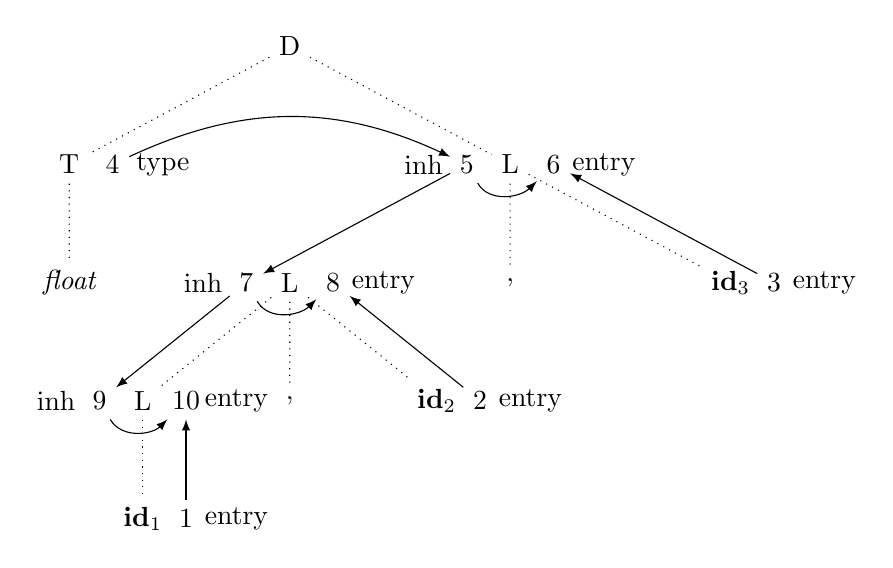
\begin{tikzpicture}[
  level/.style={sibling distance=5.6cm/#1},
  emph/.style={edge from parent/.style={dotted,draw}},
  norm/.style={edge from parent/.style={solid,draw}}
  ]
  \node (NRoot) {D}
  child[emph] {
    node (N1L) {T}
    child {
      node (N1L2) {\it float}
    }
  }
  child[emph] {
    node (N1R) {L}
    child {
      node (N1R2L) {L}
      child {
        node (N1R2L3L) {L}
        child {
          node (N1R2L3L4) {\(\textbf{id}_{1}\)}
        }
      }
      child {
        node (N1R2L3M) {\(,\)}
      }
      child {
        node (N1R2L3R) {\(\textbf{id}_{2}\)}
      };
    }
    child {
      node (N1R2M) {\(,\)}
    }
    child {
      node (N1R2R) {\(\textbf{id}_{3}\)}
    }
  };

  \path (N1L) ++(0.55,0) node (N1Lsyn) {4} -- ++(0.64,0) node {type};
  \path (N1R) ++(-0.55,0) node (N1Rinh) {5} -- ++(-0.55,0) node {inh};
  \path (N1R) ++(0.55,0) node (N1Rsyn) {6} -- ++(0.64,0) node {entry};
  \path (N1R2L) ++(-0.55,0) node (N1R2Linh) {7} -- ++(-0.55,0) node {inh};
  \path (N1R2L) ++(0.55,0) node (N1R2Lsyn) {8} -- ++(0.64,0) node {entry};
  \path (N1R2L3L) ++(-0.55,0) node (N1R2L3Linh) {9} -- ++(-0.55,0) node {inh};
  \path (N1R2L3L) ++(0.55,0) node (N1R2L3Lsyn) {10} -- ++(0.64,0) node {entry};
  \path (N1R2L3L4) ++(0.55,0) node (N1R2L3L4syn) {1} -- ++(0.64,0) node {entry};
  \path (N1R2L3R) ++(0.55,0) node (N1R2L3Rsyn) {2} -- ++(0.64,0) node {entry};
  \path (N1R2R) ++(0.55,0) node (N1R2Rsyn) {3} -- ++(0.64,0) node {entry};

  \path[-latex,black,draw]
  (N1R2L3L4syn) edge                 (N1R2L3Lsyn)
  (N1R2L3Rsyn)  edge                 (N1R2Lsyn)
  (N1R2Rsyn)    edge                 (N1Rsyn)
  (N1Rinh)      edge                 (N1R2Linh)
  (N1R2Linh)    edge                 (N1R2L3Linh)
  (N1Lsyn)      edge[out=25,in=155]  (N1Rinh)
  (N1Rinh)      edge[out=300,in=225] (N1Rsyn)
  (N1R2Linh)    edge[out=300,in=225] (N1R2Lsyn)
  (N1R2L3Linh)  edge[out=300,in=225] (N1R2L3Lsyn)
  ;
\end{tikzpicture}
\end{document}
